% \documentclass[../main.tex]{subfiles}

% \begin{document}

{
\setstretch{1.0}
\chapter{Localisation of three sex-related genes and the germline marker \textit{Vasa}/Vasa in the early developmental stages of \textit{Mytilus galloprovincialis}}
\label{chapter4}

\noindent{\large{Filippo Nicolini\textsuperscript{1,2}, Sergey Nuzhdin\textsuperscript{3}, Fabrizio Ghiselli\textsuperscript{1}, Andrea Luchetti\textsuperscript{1}, Liliana Milani\textsuperscript{1}}}

\vspace{5mm}

\noindent{\textsuperscript{1}\textit{Department of Biological, Geological and Environmental Science, University of Bologna, Bologna (BO), Italy}.}

\noindent{\textsuperscript{2}\textit{Fano Marine Center, Fano (PU), Italy}.}

\noindent{\textsuperscript{3}\textit{3Department of Molecular and Computational Biology, University of Southern California, Los Angeles, CA, USA}.}

\vspace{5mm}

\noindent{\large{\textbf{\textit{In preparation.}}}}
}

\newpage

\section{Introduction} \label{chapter4_introduction}

Despite the huge socio-economic and scientific importance of bivalves, the knowledge concerning the genetic and molecular bases of their \gls{sd} system is scarce and overlooked (\citebold{breton2018sex, nicolini2023bivalves}). Several components of the \gls{dsfg} families have been appointed as directly involved in \gls{sd} by many works, mainly thanks to \gls{dge} analyses (e.g., \citebold{milani2013nuclear, zhang2014genomic, capt2018deciphering, shi2018proteome}), mRNA/protein visualisation (REFERENCE REFERENCE REFERENCE), \gls{rnai} (REFERENCE REFERENCE REFERENCE) and \gls{qrt-pcr} (\citebold{liang2019sox2,sun2022examination}). For example, \citeboldyearparent{li2018foxl2} found that \textit{Fox-L2} and \gls{dmrt-1l} are predominantly transcribed in ovaries and testes, respectively, of the Yesso scallop \gls{pyes}, and that they contribute to establish the sexual identity of immature follicles at the molecular level prior to the morphological level. \citeboldyearparent{liang2019sox2} showed that \textit{Sox-2} is involved in the differentiation of male gonads and spermatogenesis of the scallop \gls{cfar}, and that the knocked-out phenotype results in severe loss of both germ-cell mass and spermatogonia. \citeboldyearparent{wang2020identification} speculated that \textit{Fox-L2} is involved in the sex differentiation of female gonads in the freshwater mussel \gls{hcum}. Overall, considerable effort has been made to characterise the transcription patterns of \glspl{dsfg} of interest during the adult stage of bivalves, covering various reproductive phases, while little attention has been given to the embryo and larval stages. Nonetheless, early animal development may represent a crucial moment to the establishment of the sexual identity, as the transcription of \glspl{srg} and \gls{sd} itself begins much earlier than the onset of gonad development and differentiation (even as early as the zygote formation; \citebold{richardson2023comparativeSex}). In mammals, for example, the transcription of \glspl{srg} can be detected during the embryo preimplantation stage (before \qty{4.5}{\dpf}; reviewed in \citebold{richardson2023comparativeSex}), while \gls{sry} realises its function as the male \gls{sdg} at 10.5 days post coitum (\citebold{beukeboom2014evolution}). In \gls{dmel}, the early female splicing variant of \gls{sxl}---which is the top regulator of the \gls{sd} cascade and is activated by a mechanism of chromosome counting (\textbf{\textit{inset}} in \cref{fig:DSFG_testDivergence-D}), is transcribed during the syncytial stages of the embryo (i.e., before \qty{2}{\hpf}; \citebold{salz2010sex}), when it establishes the sexual identity of the embryo through a cell-autonomous mechanism. Therefore, the study of bivalve \gls{sd} necessarily requires to consider also the early stages of embryonic and larval development, in order to obtain a comprehensive scenario of the process. Among bivalves, several species may constitute a model system particularly suitable to study the \gls{sd} process during embryogenesis, because of the presence of the \gls{dui} of mitochondria. This process---which involves the uniparental transmission of the maternal and paternal mitochondrial genomes through eggs and sperm, respectively, allows for an \textit{a-priori} detection of the sexual identity of developing embryos, as early as the first cleavage division of the zygote: in female embryos, the sperm-inherited mitochondria assume a dispersed pattern between blastomeres; conversely, in males the sperm-inherited mitochondria stay assembled together, remain within one blastomere, and are eventually included in \glspl{pgc} (\citebold{zouros2013biparental,ghiselli2019natural}).

Here we sought to expand the knowledge on the process of bivalve \gls{sd}, by employing the Mediterranean mussel \gls{mgal} as a study system, which is a species exhibiting \gls{dui}. Particularly, we aimed to investigate the transcription patterns of three \gls{dsfg} (namely, \pac{dmrt-1l}, \textit{Sox-H}, and \textit{Fox-L2}) during embryo and early larval stages. To this purpose, (i) we first performed a time-series \gls{dge} analysis by using the RNA-sequencing data published by \citeboldyearparent{miglioli2024hcrMytilus}; afterwards, (ii) we investigated the temporal and spatial transcription patterns of the \glspl{dsfg} of interest through mRNA \textit{in-situ} \gls{hcr}. To obtain a more comprehensive developmental context for the transcription patterns of \glspl{dsfg}, (iii) we also traced for the first time in \gls{mgal} the process of the germline specification through mRNA \textit{in-situ} \gls{hcr} and immunolocalization of \textit{Vasa}/Vasa, which is a traditionally-recognised marker of \glspl{pgc} and \glspl{gc} across Metazoa (\citebold{extavour2003mechanisms}). The specification and differentiation of \glspl{gc} (which are part of the gonadal tissue in adults) is in fact a critical process in sexually reproducing multicellular organisms, as it provides the groundwork for the subsequent differentiation of sexually dimorphic gametes. Therefore, understanding the developmental pathway leading to the establishment of \glspl{pgc} and \glspl{gc} is essential to fully characterise the sex-determining process and how the sexual fate of \glspl{pgc}/\glspl{gc} is directed.

\section{Materials and Methods} \label{chapter4_MM}
\subsection{Time-series gene expression}
\citeboldyearparent{miglioli2024hcrMytilus} recently produced one of the very first detailed developmental transcriptomes of the Mediterranean mussel \gls{mgal}, spanning from the unfertilized oocyte to the larval stage at \qty{72}{\hpf}, with time points sampled every \qty{4}{\hpf}. A total of thirty different mRNA libraries was sequenced, consisting of fifteen developmental time points per two biological replicates each (\cref{suppTab:readMappings}). These data are extremely useful to thoroughly investigate the transcription patterns of genes throughout the first three days of the \gls{mgal} development, to quantify the transcription level of target genes to be investigated with mRNA \gls{hcr} experiments and to have an overview of the possible outcome from such analysis.

Raw reads were downloaded from the Sequence Read Archive (SRA) in NCBI (BioProject: PRJNA996031) and trimmed using Trimmomatic v0.39 (\citebold{bolger2014trimmomatic}; \verb|LEADING:5| \verb|TRAILING:5 SLIDINGWINDOW:4:15 MINLEN:65|). Read quality was checked using FastQC v0.12.1 (\citebold{andrews2010fastqc}). Trimmed reads were mapped against the \gls{mgal} annotated genome (GCA\_900618805.1; \citebold{gerdol2020massive}) using STAR v2.7.10b (\citebold{dobin2013star}) in ‘alignReads’ mode with default parameters. The resulting gene count matrix was extracted with StringTie v2.2.1 (\citebold{pertea2015stringtie,pertea2016stringtie}) in expression estimation mode followed by the python script ‘prepDE.py’ (\verb|-l 99|).

The resulting matrix was processed in R. Raw gene counts were normalised using the median of ratios method as implemented by the DESeq2 package (\citebold{love2014deseq2}), and then transformed through the DESeq2 variance stabilising transformation (vst). Transformed gene counts were used to run a \gls{pca} and visualise sample clustering, and to plot expression values of \textit{Vasa}, \gls{dmrt-1l}, \textit{Sox-H}, and \textit{Fox-L2} (hereafter collectively referred to as ‘target genes’). Normalised gene counts were instead used to run a time-series \gls{dge} analysis in ‘maSigPro’ (\citebold{conesa2006masigpro}).

The entire pipeline was automated through custom python and bash scripts, which are available in a private repository on GitHub.

\subsection{Sample collection, MitoTracker staining and fixation}
Adult mussels were hand collected from various locations surrounding the AltaSea institute at the port of Los Angeles (CA, USA). Sampling took place during the spawning season of the species in California, i.e., from October 2023 to early January 2024.

Selected mussels were thoroughly cleaned from epibionts and placed in ice for approximately 30--60 minutes, then transferred in \gls{fasw} at \qty{16}{\degreeCelsius} and acclimatised for 30 minutes. All the individuals were then placed in a common tank and spawning was induced by cyclical thermal shock, that is, by exposing mussels alternatively to \gls{fasw} at \qtyrange{24}{26}{\degreeCelsius} and \qtyrange{14}{16}{\degreeCelsius} for a time of \qtyrange{30}{40}{\minute} each. As soon as mussels started spawning, individuals were promptly removed from the common tank, carefully washed, air dried to remove contaminant gametes from the shell, and then allowed to continue spawning in isolated containers of about \qty{250}{\ml} with \qty{16}{\degreeCelsius} \gls{fasw}.

Both single and multiple crosses were performed: two males (M1, M2) and two females (F1, F2) were employed for single crosses; six males and six females were employed for multiple crosses, and gametes from the same sex were mixed. One hour after the spawning started, oocytes were filtered through a \num{75} over a \qty{30}{\um} mesh, and aged in \qty{1}{\l} of \gls{fasw} for \qtyrange{40}{60}{\minute}, to allow them to assume a proper circular shape. Oocyte abundance was estimated under a stereomicroscope by eye counting the number of gametes in five aliquots of \qty{1}{\ml}, and then calculating the mean value. Sperm mitochondria were labelled with MitoTracker Red CMXRos (Thermo Fisher Scientific) at a working concentration of \qty{500}{\nano\molar} for \qty{30}{\minute}. MitoTracker is a fluorescent, vital and fixation-resistant mitochondrial dye and was used to be able to detect the sex of developing embryos (as early as the two-blastomere stage) according to the distribution pattern of sperm mitochondria (\citebold{cao2004differential,obata2005specific}). From this step onward, samples were always kept in the dark.

Fertilisation was performed by mixing oocytes and sperm at a ratio of 1:10. Fertilisation success was checked after \qtyrange{20}{30}{\minute} by the formation of polar bodies. The suspension was then carefully washed on a \qty{30}{\um} mesh to remove excess sperm, and brought to a concentration of \qty{250}{\zygotes\per\ml}. The resulting suspension was transferred into cell-culture flasks of \qty{40}{\ml} and embryos/larvae were reared at \qty{16(1)}{\degreeCelsius} in the dark. Water was changed every \qty{24}{\hour}. After \qty{48}{\hpf}, larvae were fed with the unicellular microalgae \textit{Isochrysis galbana}, at a final concentration of about \qty{100000}{\cells\per\ml} following \citeboldyearparent{helm2004hatchery}.

Embryos/larvae were sampled at \qtylist{1;2;3;4}{\hpf}, and then every \qty{12}{\hour} until \qty{72}{\hpf}. Proper development and vitality were checked under a stereomicroscope at every sampling time. After concentration with a mesh of proper size, embryos/larvae were fixed in 3.2\% \gls{pfa} in \gls{pbs} at \qty{4}{\degreeCelsius} overnight under constant and gentle shaking. \gls{pbs} was prepared with the following concentrations: \qty{128}{\milli\molar} \ce{NaCl}, \qty{2}{\milli\molar} \ce{KCl}, \qty{8}{\milli\molar} \ce{Na2HPO4*2H2O}, and \qty{2}{\milli\molar} \ce{KH2PO4}. Fixed samples were washed 3×\qty{20}{min} in \gls{pbstw} and then dehydrated 3×\qty{30}{\minute} in absolute methanol at \gls{rt}. Dehydrated samples were stored at \qty{-20}{\degreeCelsius} until usage.

\subsection{mRNA \textit{in-situ} hybridization chain reaction (HCR)}
\subsubsection{HCR probe design}
\textit{Vasa}, \gls{dmrt-1l}, \textit{Sox-H}, and \textit{Fox-L2} (the latter three are hereafter referred to as \pac{srg}) spliced-transcript nucleotide sequences of \gls{mgal} were obtained from the previous analyses with OrthoFinder v2.5.5 (\citebold{emms2019orthofinder}) on annotated bivalve genomes and transcriptomes (see \cref{chapter3_MM}). Accession numbers of spliced transcripts are 10B017427, 10B093608, 10B014180, and 10B094018, respectively. The ‘insitu\_probe\_generator’ script from the Ozpolat Lab (\citebold{kuehn2022probegenerator}) was used to generate pairs of probes specifically designed for third-generation \gls{hcr} (\citebold{choi2018hcr3}). The built-in BLASTN search against the annotated \gls{mgal} transcriptome was employed to check for putative off-target bindings of probe pairs. B1-488, B2-647, B3-546, and B4-700 pairs of \gls{hcr} amplifiers and fluorophores were chosen, as reported in \cref{tab:fluorescent_dyes}. Resulting probes were synthesised by Integrated DNA Techonologies (IDT\texttrademark) in separate oligo pools.

\begin{table}[ht!]
    \centering
    \caption[\textbf{Characteristics of fluorescent dyes used for each labelled target}]
    {
        \textbf{Characteristics of fluorescent dyes used for each labelled target}. \gls{hcr} amplifiers and the number of probe sets (as in \cref{suppTab:HCRprobes}) are reported when applicable. Dyes for both \textit{Vasa} and Vasa are reported.
    }
    \label{tab:fluorescent_dyes}
    \begin{tabular}{llcccc}
    \toprule
    \textbf{Target}                                              & \textbf{Dye}                                                     & \textbf{\begin{tabular}[c]{@{}c@{}}HCR\\ amplifier\end{tabular}} & \multicolumn{1}{c}{\textbf{\begin{tabular}[c]{@{}c@{}}HCR\\ probe pairs\end{tabular}}} & \multicolumn{1}{c}{\textbf{\begin{tabular}[c]{@{}c@{}}Excitation\\ (nm)\end{tabular}}} & \multicolumn{1}{c}{\textbf{\begin{tabular}[c]{@{}c@{}}Emission\\ (nm)\end{tabular}}} \\* \midrule \midrule
    \begin{tabular}[c]{@{}l@{}}dsDNA\\ (nuclei)\end{tabular}                                               & DAPI                                                             & \NA                                                              & \NA                                                                                    & 360                                                                                    & 460                                                                                  \\ [0.6cm]
    \begin{tabular}[c]{@{}l@{}}Sperm\\ mitochondria\end{tabular}                                           & \begin{tabular}[c]{@{}l@{}}MitoTracker\\ Red CMXRos\end{tabular} & \NA                                                              & \NA                                                                                    & 575                                                                                    & 600                                                                                  \\ [0.6cm]
    \textit{Vasa}/Vasa & ALEXA-488/-488    & B1/\NA                  & 33/\NA                                        & 499                                                                                    & 520                                                                                  \\* [0.3cm]
    \textit{Dmrt-1L}                                             & ALEXA-647                                                        & B2                                                               & 18                                                                                     & 653                                                                                    & 670                                                                                  \\ [0.3cm]
    \textit{Sox-H}                                               & ALEXA-546                                                        & B3                                                               & 22                                                                                     & 557                                                                                    & 575                                                                                  \\ [0.3cm]
    \textit{Fox-L2}                                              & ALEXA-700                                                        & B4                                                               & 28                                                                                     & 685                                                                                    & 700                                                                                 \\* \bottomrule \bottomrule
    \end{tabular}
    \end{table}

\subsubsection{mRNA \textit{in-situ} HCR and microscope imaging}
mRNA \textit{in-situ} \gls{hcr} in \gls{mgal} embryos was performed following \citeboldyearparent{miglioli2024hcrMytilus}. All the steps were carried out in the dark to prevent MitoTracker from fading. Probe hybridization buffer, probe wash buffer and amplification buffer were manufactured by Molecular Instruments, Inc.

Dehydrated samples stored in methanol were washed 4×\qty{5}{\minute} and 1×\qty{10}{\minute} in \gls{pbstw}. Samples were then permeabilized for \qty{30}{\minute} in a detergent solution (1.0\% sodium dodecyl sulfate [SDS], 0.5\% Tween 20, \qty{50}{\milli\molar} \ce{Tris-HCl}, \qty{1}{\milli\molar} ethylenediaminetetraacetic acid (EDTA), \qty{150}{\milli\molar} \ce{NaCl}), and washed again 2×\qty{5}{\minute} in \gls{pbstw}. Samples were prepared for the \gls{hcr} detection stage by incubation in the probe hybridization buffer for \qty{30}{\minute} at \qty{37}{\degreeCelsius}. Detection stage was then performed with \qty{4}{\nano\molar} of each probe set in hybridization solution overnight (\qty{>12}{\hour}) at \qty{37}{\degreeCelsius}.

Excess probes were removed by washing 4×\qty{20}{\minute} with probe wash buffer at \qty{37}{\degreeCelsius} and 3×\qty{5}{\minute} with \gls{ssct} at \gls{rt}. Samples were incubated for \qty{30}{\minute} in the amplification buffer at \gls{rt}. Hairpins were heated at \qty{95}{\degreeCelsius} for \qty{90}{\second} and then snap-cooled at \gls{rt} for \qty{30}{\minute}. The amplification step of \gls{hcr} was performed with \qty{6}{\pmol} of each hairpin in the amplification buffer overnight (\qty{>12}{\hour}) at \gls{rt}.

Excess hairpins were removed by washing 2×\qty{5}{\minute}, 2×\qty{10}{\minute}, and 1×\qty{5}{\minute} with \gls{ssct}. If not immediately mounted on slides, samples were stored in \gls{ssct} at \qty{+4}{\degreeCelsius}. Otherwise, samples were immersed first in 50\% glycerol and then in 75\% glycerol, each for \qtyrange{30}{60}{\minute}, and then mounted with VECTASHIELD\textregistered PLUS Antifade Mounting Medium with DAPI (H-2000). Slides were imaged on a Stellaris 5 Confocal Package system with the software Las X (Leica Microsystems). Each dye was imaged sequentially in a separate channel, to enhance the yield and avoid crosstalks. \cref{tab:fluorescent_dyes} summarises the excitation and emission peaks for each dye. Images were then manipulated and post-produced using Fiji v2.14.0.

\subsection{Immunolocalization of Vasa}
\gls{mgal} Vasa sequence was manually inspected through multiple sequence alignment with Vasa from other bivalves (data from \cref{chapter3}) and several reference species (\gls{drer} [Ddx4: NP\_571132.1]; \gls{hsap} [Ddx4: NP\_077726.1]; \gls{mmus} [Ddx4: NP\_001139357.1]; \gls{dmel} [Vasa: NP\_001260458.1]; \gls{cele} [GLH-1: NP\_001262379.1, GLH-2: NP\_491876.1, GLH-3: NP\_491681.1, GLH-4: NP\_491207.3]), to support commercial antibody specificity in \gls{mgal}. The Vasa sequence from \gls{drer} was included as the polyclonal antibody was generated using the zebrafish protein variant (manufacturer indications; ab209710 by Abcam Limited). A \gls{ml} phylogenetic tree of Vasa genes and its paralog DDX3 (reference genes:  \gls{drer} [Ddx3Xa: NP\_001119895.1, Ddx3Xb: NP\_571016.2]; \gls{hsap} [DDX3X: NP\_001180346.1]; \gls{mmus} [Pl10/Ddx3Xl: NP\_149068.1]; \gls{dmel} [Belle: NP\_001262379.1]; \gls{cele} [LAF-1: NP\_001254859.1, VBH-1: NP\_001021793.1]) was built using IQTREE. The \gls{hmm} profile of the \gls{dead/deah-box} signature domain for the amino acid guided alignment step, was built after the corresponding Pfam full database (PF00270). Methods are the same as in \cref{chapter3}. 

Vasa immunolocalization in \gls{mgal} embryos was performed following \citeboldyearparent{milani2011doubly} with modifications. All the steps were carried out in the dark to prevent MitoTracker fluorescence from fading. Dehydrated samples stored in methanol were rinsed 3×\qty{10}{\minute} and 1×\qty{2}{\hour} in \gls{tbs}, following an additional wash for \qty{10}{\minute} with \gls{pbs}. Samples were then digested for \qty{6}{\minute} and \qty{30}{\second} with 0.01\% pronase E (Merck) in \gls{pbs}, and washed again 2×\qty{5}{\minute} in \gls{pbs}. Permeabilization was performed in \gls{tbstx} 0.1\% for \qty{5}{\minute} at \gls{rt} and in \gls{tbstx} 1\% overnight at \qty{4}{\degreeCelsius}.

After an additional rinse for \qty{5}{\minute} in \gls{tbstx} 0.1\%, non-specific binding sites were blocked with a \gls{tbstx} 0.1\% solution containing 3\% bovine serum albumin (BSA). Samples were then incubated at \qty{4}{\degreeCelsius} for \qtyrange{32}{48}{\hour} with primary anti-VASA/VAS antibody (polyclonal anti-VASA developed in rabbit; ab209710 by Abcam Limited), diluted 1:100.

Excess primary antibody was rinsed from samples with 4×\qty{30}{\minute} in \gls{tbstx} 0.1\%, followed by an incubation of \qty{1}{hour} in \gls{tbstx} 0.1\% containing 3\% BSA. Samples were then incubated at \qty{+4}{\degreeCelsius} for \qtyrange{24}{32}{\hour} with secondary antibody HRP anti-rabbit in goat (Santa Cruz Biotechnology Inc.), diluted 1:400.

Excess secondary antibody was rinsed with 4×\qty{30}{\minute} in TBS-Tx 0.1\% and 1×\qty{1}{hour} in \glossary{tbstx} 1\%. Samples were immersed first in 50\% glycerol and then in 75\% glycerol, each for \qtyrange{30}{60}{\minute}, and then mounted with VECTASHIELD\textregistered PLUS Antifade Mounting Medium with DAPI (H-2000). Slides were imaged on a Nikon A1R+ HD25 confocal microscope. Each dye was imaged sequentially in a separate channel, to enhance the yield and avoid any crosstalks. \cref{tab:fluorescent_dyes} summarises the excitation and emission peaks for each dye. Images were then manipulated and post-produced using Fiji v2.14.0.

\section{Results} \label{chapter4_results}
\subsection{Differential gene expression analysis of \textit{Vasa} and SRGs in embryo time-series} \label{chapter4_DGE}
Over 24 millions reads were mapped for each RNA-sequencing library (86.58\% of the total input reads), with an average of 26.8 millions (\cref{suppTab:readMappings}). Of these, an average of 22 millions reads were uniquely mapped (71.86\% of the total input reads), while an average of 4.5 millions were multi-mapped (14.72\% of the total input reads). The average of unmapped reads was 4.1 millions (13.42\% of the total input reads; \cref{suppTab:readMappings}). The \gls{pca} on normalised read counts returned well-clustered experimental groups for time points between \qtylist{8;36}{\hpf}, while for stages before \qty{8}{\hpf} and after \qty{36}{\hpf}, experimental groups are more homogeneous among each other (\cref{fig:deseq2-A}). This situation may reflect major developmental dynamics during embryogenesis and larval development. As a matter of fact, before \qty{8}{\hpf}, the embryo undergoes segmentation and no big morphogenetic movements are usually detected. Between \qtylist{8;13}{\hpf}, instead, gastrulation begins, the embryo experiences strong morphogenetic rearrangements (such as the formation of embryonic layers) and the trochophore larva develops, all processes which are expected to be detected also at the molecular level. After \qty{36}{\hpf}, instead, the larva does not show any dramatic morphogenetic event, as the D-veliger is almost formed and the gross advanced larval morphology is established. The hierarchical clustering of differentially expressed genes computed by \citeboldyearparent{miglioli2024hcrMytilus} is concordant with this view.

\begin{figure}[t!]
	\centering
	\captionsetup[subfigure]{labelformat=nocaption}
	\begin{subfigure}{0\linewidth}
	\caption{}\label{fig:deseq2-A}
	\end{subfigure}% <----- get rid of space, for proper centering
	\begin{subfigure}{0\linewidth}
	\caption{}\label{fig:deseq2-B}
	\end{subfigure}% <----- get rid of space, for proper centering
    \includegraphics[width=\textwidth]{chapter4/figure_1.png}
	\caption[\textbf{\gls{pca} of DESeq2-normalised read counts (A) and transcription levels of target and reference genes (B)}]
	{
		\textbf{\gls{pca} of DESeq2-normalised read counts (A) and transcription levels of target and reference genes (B)}. (A) Principal components (PC) 1 and 2 are plotted in the x and y axes, respectively; the proportion of variance explained by each PC is shown in parentheses. Sampled time-points are shown in different colours and are indicated by the hours \glsxtrfull{hpf}. Major developmental transitions are marked with dotted lines. \gls{pca} has been performed on vst-transformed, normalised read counts (DESeq2 median of ratios). (B) Transcription levels of target (\textit{Vasa}, \gls{dmrt-1l}, \textit{Sox-H}, and \textit{Fox-L2}) and reference genes (\textit{Wnt-8a} and \textit{Fox-B2}) as expressed by normalised read counts (DESeq2 median of ratios).
	}
	\label{fig:deseq2}
\end{figure}

Transcription levels of \textit{Vasa}, \glspl{srg}, \textit{Fox-B2}, and \textit{Wnt-8a} were plotted individually (\cref{fig:deseq2-B}) to obtain a proxy of the expected outcome of \gls{hcr}. \textit{Fox-B2} and \textit{Wnt-8a} were employed as control genes to get support for handling of data and of the pipeline, as they were also analysed by \citeboldyearparent{miglioli2024hcrMytilus}. The transcription of both genes starts at \qtylist{4;8}{\hpf}, respectively, reaches a peak at \qty{16}{\hpf}, and then constantly decreases ({fig:deseq2-B}). \textit{Vasa} transcripts are highly abundant in unfertilized oocytes and in embryos \qty{4}{\hpf}, then constantly decrease throughout time; conversely, \textit{Fox-L2} transcripts increase from \qty{12}{\hpf} onward ({fig:deseq2-B}). Both \gls{dmrt-1l} and \textit{Sox-H}, instead, show low or null levels of transcriptions throughout the entire time series ({fig:deseq2-B}).

The maSigPro \gls{dge} analysis of the \gls{mgal} developmental time series found \num{13067} differentially expressed genes (about 17\% of the analysed genes) and clustered them into 9 different groups, according to their specific transcriptional profiles (\cref{fig:masigpro}). Among the genes of interest, only \textit{Vasa} and \textit{Fox-L2} showed a significantly different transcriptional profile throughout the time series, and were included in clusters 3 and 1, respectively. As already discussed, \textit{Vasa} and \textit{Fox-L2} transcription levels show an opposite tendency, with the former decreasing and the latter increasing throughout time. Both \gls{dmrt-1l} and \textit{Sox-H} were not found to be differentially transcribed by maSigPro and, thus, were not included in any cluster. The same holds true for \textit{Wnt-8a} and \textit{Fox-B2}.

\begin{figure}[t!]
	\centering
	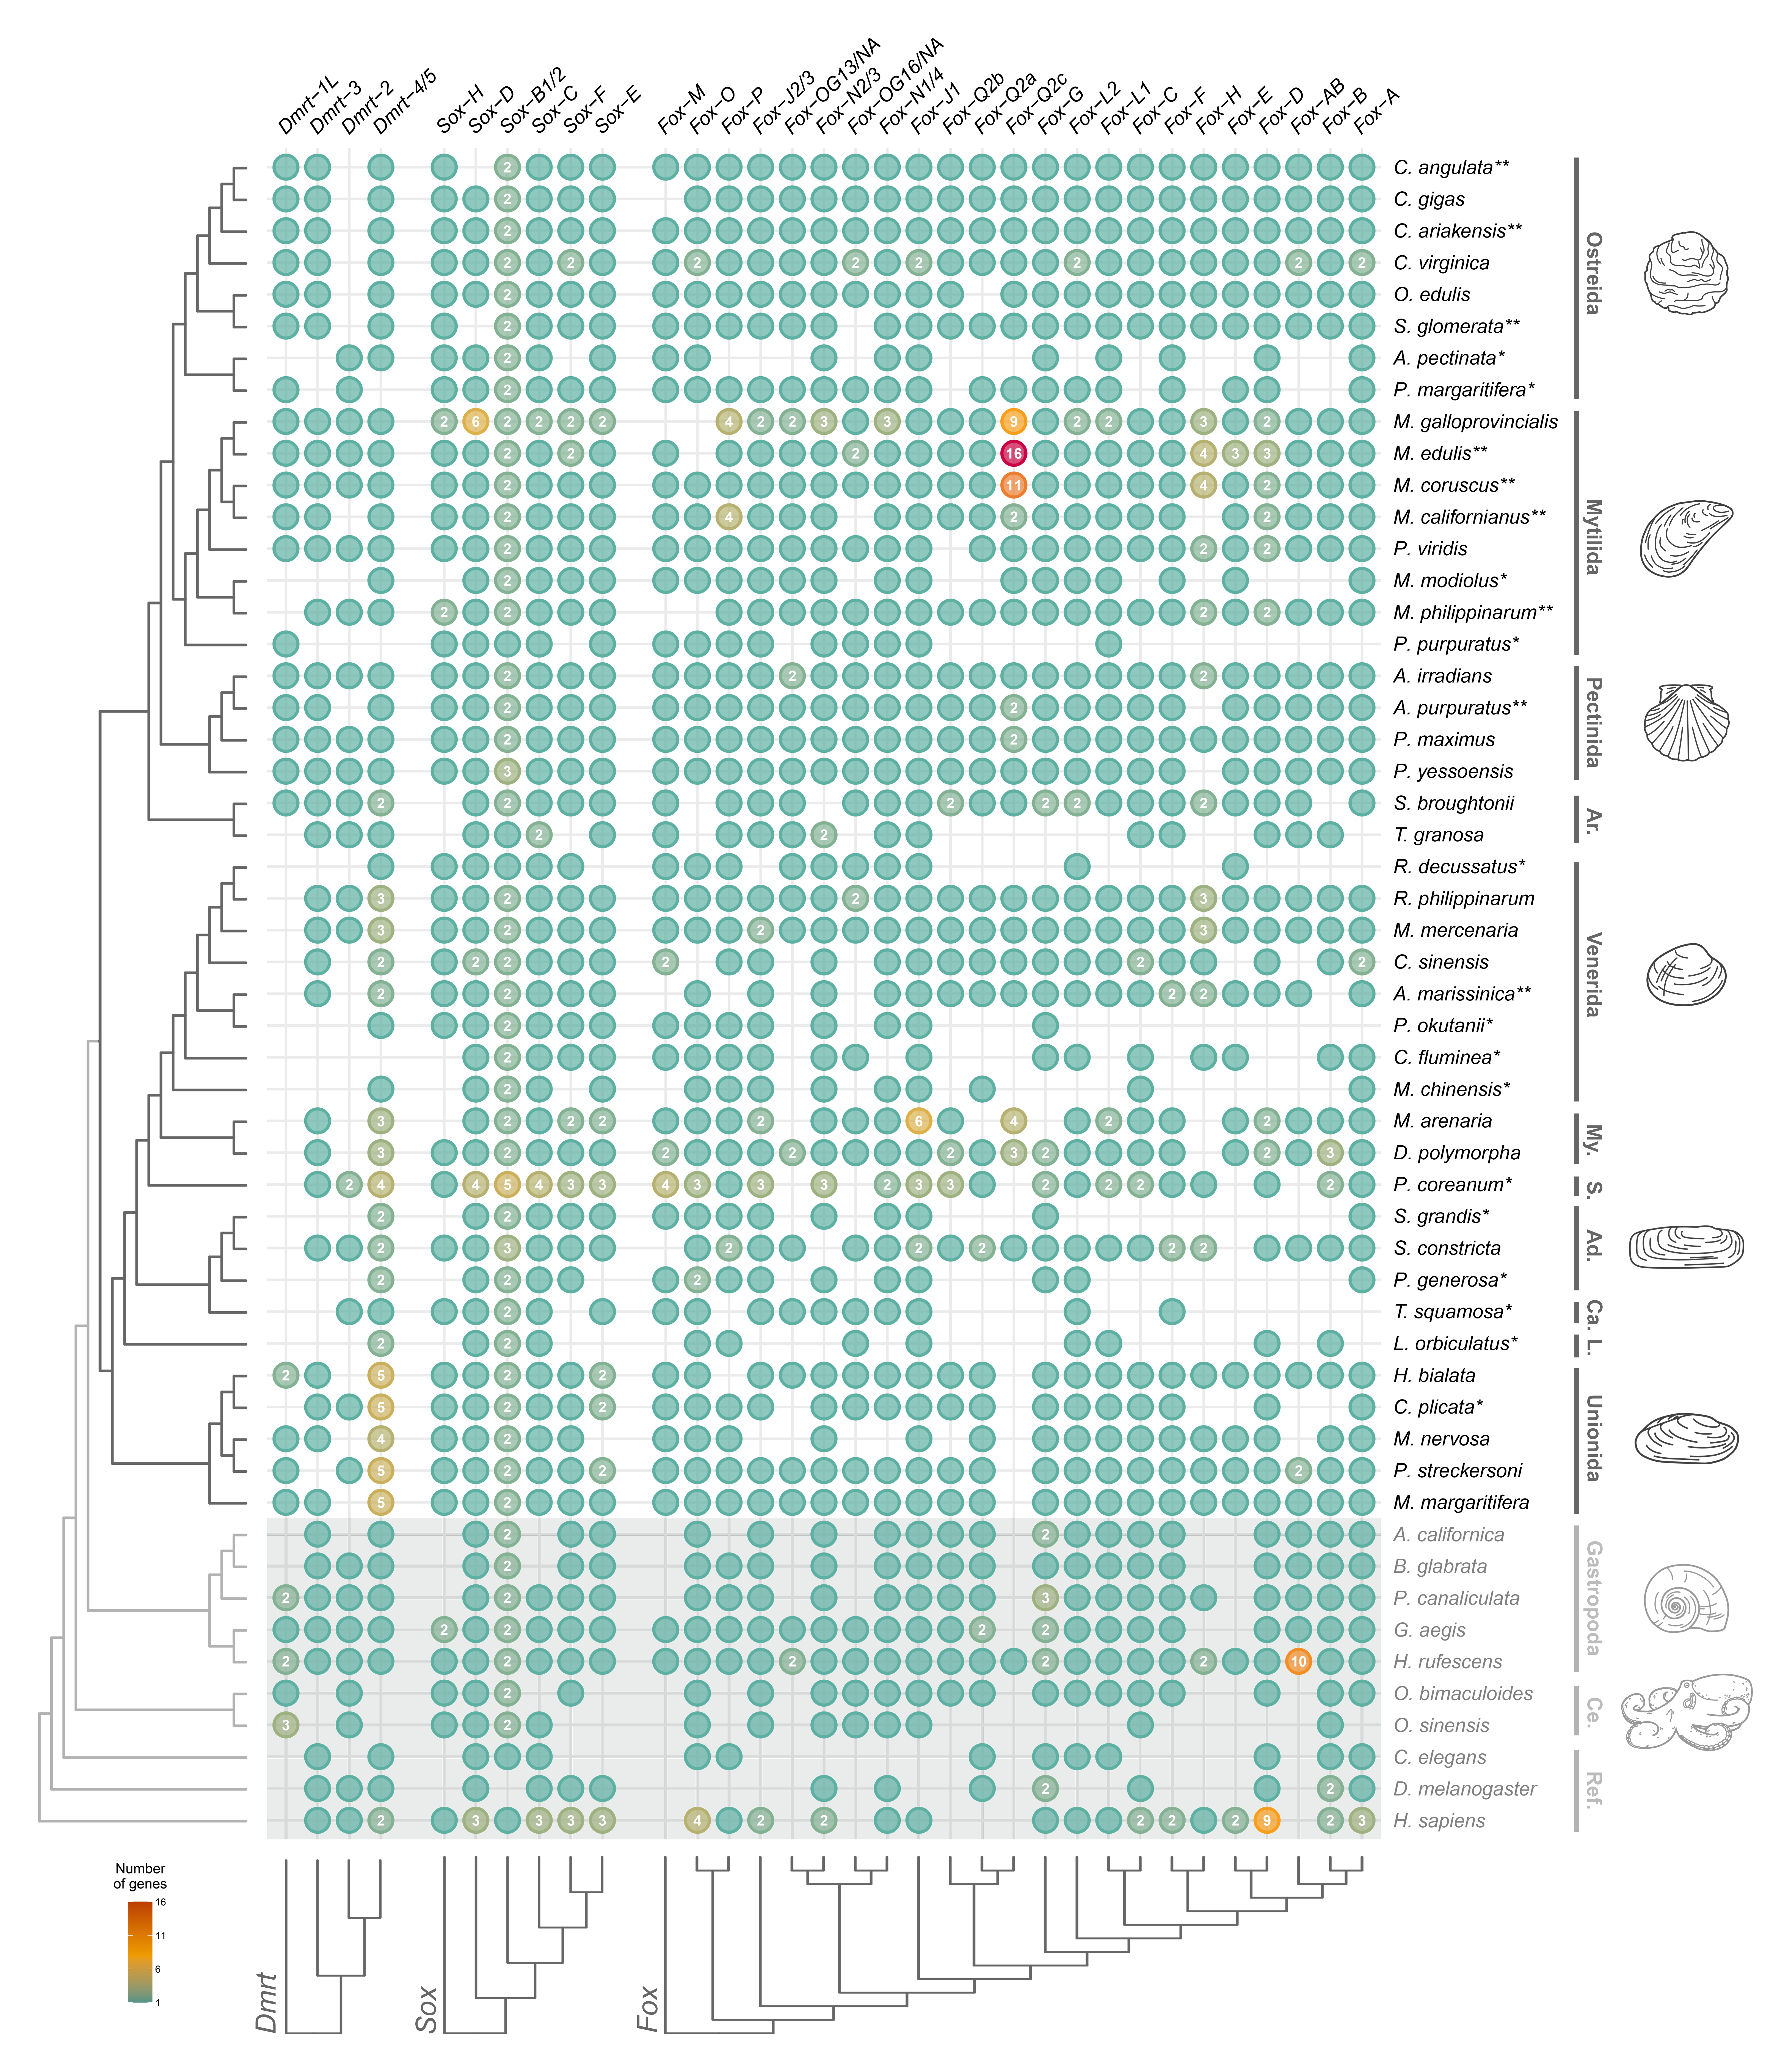
\includegraphics[width=\textwidth]{chapter4/figure_2.png}

	\caption[\textbf{Transcription patterns of differentially-expressed genes as inferred by maSigPro}]
	{
		\textbf{Transcription patterns of differentially-expressed genes as inferred by maSigPro}. Genes are divided into 9 different clusters according to their transcription patterns throughout 15 sampled time points. Median values of the two biological replicates are shown for each time point and represented by points. Mean values are shown for each time point and represented by solid lines.
	}
	\label{fig:masigpro}
\end{figure}

\subsection{mRNA \textit{in-situ} HCR of \textit{Vasa} and SRGs}
Overall, a total of 80 adult \gls{mgal} individuals were sampled and staged for thermal-shock induced spawning. Of these, 8 males and 8 females were eventually selected as parents for single (2 of each sex) and multiple (6 of each sex) crosses, on the basis of their gamete quality (i.e., presence sperm motility, and oocyte transparency and rounded shape). MitoTracker labelling was successfully retained in developing embryos of \gls{mgal} until \qty{12}{\hpf}. After that stage, the stained sperm mitochondria were difficult to detect, and so was the dispersal pattern to establish the sexual identity.

After embryo rearing, fixation, and mRNA \textit{in-situ} \gls{hcr} of target genes, a total of 16 oocytes, 81 embryos and 33 mussel larvae were imaged (\cref{tab:embryo_count}). Of these, on the basis of sperm mitochondria dispersal patterns, 55 were females (dispersed pattern), 28 were males (aggregated pattern) and 38 were of indeterminable sex (ambiguous pattern or unlabelled sperm mitochondria). For each stage, negative controls were also imaged (final count of 36), by staining just sperm mitochondria with MitoTracker and nuclei with DAPI, and going through the \gls{hcr} protocol without adding probes in the hybridization step. Overall, a total of 137 samples were imaged.

\begin{table}[t!]
    \centering
    \caption[\textbf{Number of imaged samples, divided by developmental stage, experiment, and sex}]
    {
        \textbf{Number of imaged samples, divided by developmental stage, experiment, and sex}.
    }
    \label{tab:embryo_count}
    \begin{tabular}{llrrrr}
        \toprule
        \textbf{Stage}                & \textbf{Experiment}               & \textbf{Females} & \textbf{Males} & \textbf{Undetermined} & \textbf{Total} \\* \midrule \midrule
        \textbf{Oocytes}              & \textbf{HCR} & \NA     & \NA   & \NA          & \textbf{11}    \\* \midrule
        2-cell embryos       & HCR          & 8                & 9              & 1                     & 18             \\
        4-cell embryos                & HCR          & 9                & 3              & 0                     & 12             \\
        8-cell embryos                & HCR          & 11               & 3              & 0                     & 14             \\
        12-hpf embryos                & HCR          & 7                & 6              & 0                     & 13             \\
        \textbf{Total embryos}        & \textbf{HCR} & \textbf{35}      & \textbf{21}    & \textbf{1}            & \textbf{57}    \\* \midrule
        24-hpf larvae                 & HCR          & 0                & 1              & 11                    & 12             \\
        48-hpf larvae                 & HCR          & 0                & 0              & 11                    & 11             \\
        72-hpf larvae                 & HCR          & 1                & 1              & 8                     & 10             \\
        \textbf{Total larvae}         & \textbf{HCR} & \textbf{1}       & \textbf{2}     & \textbf{30}           & \textbf{33}    \\* \midrule
        \textbf{Oocytes}              & \textbf{Negative control}         & \NA     & \NA   & \NA          & \textbf{5}     \\* \midrule
        2-cell embryos                & Negative control                  & 7                & 2              & 0                     & 9              \\
        4-cell embryos                & Negative control                  & 7                & 2              & 0                     & 9              \\
        8-cell embryos                & Negative control                  & 5                & 1              & 0                     & 6              \\
        12-hpf embryos                & Negative control                  & 0                & 0              & 3                     & 3              \\
        \textbf{Total embryos}        & \textbf{Negative control}         & \textbf{19}      & \textbf{5}     & \textbf{3}            & \textbf{27}    \\* \midrule
        \textbf{Total larvae}         & \textbf{Negative control}         & \textbf{0}       & \textbf{0}     & \textbf{4}            & \textbf{4}     \\* \midrule \midrule
        \textbf{\begin{tabular}[c]{@{}l@{}}Total imaged\\ samples\end{tabular}} & \textbf{All}                      & \textbf{55}      & \textbf{28}    & \textbf{38}           & \textbf{137}  \\* \bottomrule \bottomrule
    \end{tabular}
\end{table}

The ‘insitu\_probe\_generator’ script (\citebold{kuehn2022probegenerator}) generated: (i) 33 probe pairs conjugated with hairpin B1 and ALEXA-488 for \textit{Vasa}; (ii) 32 probe pairs conjugated with hairpin B2 and ALEXA-647 for \gls{dmrt-1l}; (iii) 27 probe pairs conjugated with hairpin B3 and ALEXA-546 for \textit{Sox-H}; and (iv) 28 probe pairs conjugated with hairpin B4 and ALEXA-700 for \textit{Fox-L2} (\cref{tab:fluorescent_dyes,suppTab:HCRprobes}).

\gls{hcr} labelling of genes of interest proved to be concordant with results obtained from RNA-seq analysis (see \cref{chapter4_DGE}). Concerning \textit{Vasa}, it has been detected throughout every sampled stage (Fig. 3A): transcripts were identified quite homogeneously in the cytoplasm of unfertilized oocytes, 2-, 4-, and 8-cell embryos; in gastrulae, \textit{Vasa} is located mainly in the ingressed cells; in trochophores, it forms a cup-like structure in the region opposite to the shell-field; in D-larvae, it is mainly retained in two central areas adjacent to the valves (right and left sides of the larvae) in a sort of a comma-shaped region. Concerning \gls{dmrt-1l} (Fig. 3B), final images were quite noisy and showed putative non-specific staining at the level of embryo external surface and larvae shell, which may have interfered with the true signal of \gls{hcr} for this gene; in any case, no clear labelling distribution pattern was found in embryos of both sexes. \textit{Sox-H} mRNAs (Fig. 3C) were not detected during the imaged developmental stages. Conversely, \textit{Fox-L2} transcripts have been detected starting from the 8-cell stage—where they are homogeneously present, to the D-veliger larvae—where they appear to be mostly co-localized with Vasa (Fig. 3D–E). Imaging of control samples (i.e., without mRNA \textit{in-situ} staining) can be found in Supp. Fig. S1.

\section{Discussion} \label{chapter4_discussion}

\textbf{\textit{In preparation.}}

% \end{document}
